\documentclass[
  bibliography=totoc,     % Literatur im Inhaltsverzeichnis
  captions=tableheading,  % Tabellenüberschriften
  titlepage=firstiscover, % Titelseite ist Deckblatt
	11pt  % font size
]{scrartcl} % Alternative: scrreprt und scrbook

% Paket float verbessern
\usepackage{scrhack}

% Warnung, falls nochmal kompiliert werden muss
\usepackage[aux]{rerunfilecheck}

% unverzichtbare Mathe-Befehle
\usepackage{amsmath}
% viele Mathe-Symbole
\usepackage{amssymb}
% Erweiterungen für amsmath
\usepackage{mathtools}
\usepackage{dsfont}
% Fonteinstellungen
\usepackage{fontspec}
% Latin Modern Fonts werden automatisch geladen
% Alternativ:
%\setromanfont{Libertinus Serif}
%\setsansfont{Libertinus Sans}
%\setmonofont{Libertinus Mono}

% Wenn man andere Schriftarten gesetzt hat, sollte man
% das Seiten-Layout neu berechnen lassen
\recalctypearea

% Rändermaße
\usepackage[
    left=3cm,
    right=3cm,
    top=1.5cm,
    bottom=2cm,
    includeheadfoot
]{geometry}

% deutsche Spracheinstellungen
\usepackage{polyglossia}
\setmainlanguage{german}


\usepackage[
  math-style=ISO,    % ┐
  bold-style=ISO,    % │
  sans-style=italic, % │ ISO-Standard folgen
  nabla=upright,     % │
  partial=upright,   % ┘
  warnings-off={           % ┐
    mathtools-colon,       % │ unnötige Warnungen ausschalten
    mathtools-overbracket, % │
  },                       % ┘
]{unicode-math}

% traditionelle Fonts für Mathematik
\setmathfont{Latin Modern Math}
% Alternativ:
%\setmathfont{Libertinus Math}

\setmathfont{XITS Math}[range={scr, bfscr}]
\setmathfont{XITS Math}[range={cal, bfcal}, StylisticSet=1]

% Zahlen und Einheiten
\usepackage[
  locale=DE,                   % deutsche Einstellungen
  separate-uncertainty=true,   % immer Fehler mit \pm
  per-mode=symbol-or-fraction, % / in inline math, fraction in display math
]{siunitx}

% chemische Formeln
\usepackage[
  version=4,
  math-greek=default, % ┐ mit unicode-math zusammenarbeiten
  text-greek=default, % ┘
]{mhchem}

% richtige Anführungszeichen
\usepackage[autostyle]{csquotes}

% schöne Brüche im Text
\usepackage{xfrac}

% Standardplatzierung für Floats einstellen
\usepackage{float}
\floatplacement{figure}{htbp}
\floatplacement{table}{htbp}

% Floats innerhalb einer Section halten
\usepackage[
  section, % Floats innerhalb der Section halten
  below,   % unterhalb der Section aber auf der selben Seite ist ok
]{placeins}

% Seite drehen für breite Tabellen: landscape Umgebung
\usepackage{pdflscape}

% Captions schöner machen.
\usepackage[
  labelfont=bf,        % Tabelle x: Abbildung y: ist jetzt fett
  font=small,          % Schrift etwas kleiner als Dokument
  width=0.9\textwidth, % maximale Breite einer Caption schmaler
]{caption}
% subfigure, subtable, subref
\usepackage{subcaption}

% Grafiken können eingebunden werden
\usepackage{graphicx}
% In folgenden Ordnern wird nach den Graphiken gesucht
\graphicspath{
  {images/}{../images/}
  {pics/}{../pics}
  {content/}{../content/}
  {build/}{../build/}
  {rohdaten/}{../rohdaten/}
  {python/}{../python}
}

% größere Variation von Dateinamen möglich
\usepackage{grffile}
% verhindert das Bilder in anderen Sections auftrerten
\usepackage{placeins}

% schöne Tabellen
\usepackage{booktabs}

% Verbesserungen am Schriftbild
\usepackage{microtype}

% Literaturverzeichnis
\usepackage[
  backend=biber,
]{biblatex}
% Quellendatenbank
\addbibresource{src.bib}
\addbibresource{programme.bib}

% Hyperlinks im Dokument
\usepackage[
  unicode,        % Unicode in PDF-Attributen erlauben
  pdfusetitle,    % Titel, Autoren und Datum als PDF-Attribute
  pdfcreator={},  % ┐ PDF-Attribute säubern
  pdfproducer={}, % ┘
]{hyperref}
% erweiterte Bookmarks im PDF
\usepackage{bookmark}

% Trennung von Wörtern mit Strichen
\usepackage[shortcuts]{extdash}

\author{
  Patrick Schmidt
  \texorpdfstring{
    \\
    \href{mailto:patrick7.schmidt@udo.edu}{patrick7.schmidt@udo.edu}
  }{}
  \texorpdfstring{\and}{, }
  Karl Schiller
  \texorpdfstring{
    \\
    \href{mailto:karl.schiller@udo.edu}{karl.schiller@udo.edu}
  }{}
}

% keine Lücke am Beginn eines Absatzes lassen
\setlength{\parindent}{0pt}
% Zwischen den Absätzen eine Leerzeile einbauen
\setlength{\parskip}{\baselineskip}

% Füllwort bei SIrange verändern
\sisetup{mode=text,range-phrase={\text{ bis }}}
% Neue Buchstaben bei SIunitx
\sisetup{math-micro=\text{µ},text-micro=µ}

% Bilder von Text umfließen lassen
\usepackage{wrapfig}

% Ermögliche Befehl \mean für einen Mittelwert
\newcommand*\mean[1]{\bar{#1}}

%% EOF %%


\subject{VERSUCH NUMMER 27}
\title{Der Zeeman-Effekt}
\date{
  \begin{flushleft}
    \hspace{4em}
    Durchführung:
    \hspace{7em}
    Abgabe: \\
    \hspace{3em}
    26. Dezember 2018
    \hspace{4em}
    \today
  \end{flushleft}
}

\begin{document}

\thispagestyle{empty}
\maketitle
\thispagestyle{empty}
\tableofcontents
\newpage
\setcounter{page}{1}

\section{Zielsetzung}
\label{sec:Zielsetzung}

Ziel des Versuches ist die Bestimmung der Diffusionskonstante von Wasser.
Diese wird mittels gepulster Kernspinresonanz (NMR) ermittelt,
indem also der zeitliche Verlauf einer Magnetisierung der Probe unter
Einstrahlung eines Hochfrequenzfeldes untersucht wird.
Dabei treten Relaxationsprozesse auf, die unter Verwendung zweier
Relaxationszeiten charakterisiert werden.

\section{Theorie}
\label{sec:Theorie}

\subsection{Magnetisierung einer Probe}
\label{sec:TheoMagnetisierung}

Im Folgenden wird die Magnetisierung einer Probe erläutert, die im thermischen
Gleichgewicht mit ihrer Umgebung steht.
Anschließend wird auf die Larmor-Präzession näher eingegangen.

Beim Anlegen eines externen Magnetfelds $\vec{B} = B_0 \vec{e}_\text{B}$ eines ansonsten
feldfreien Raums spalten die Kernspinzustände der Probe in $2S+1$ Unterniveaus auf.
Dabei zeige das Magnetfeld in $z$-Richtung und $S$ bezeichne die Spinquantenzahl der
Zustände, die mittels der Orientierungsquantenzahl $m$ unterschieden werden.
Im thermischen Gleichgewicht sind die Zustände nach der Maxwell-Boltzmann-Verteilung
und damit ungleichmäßig besetzt.
Aufgrund der Orientierung der einzelnen Spins ergibt sich daraus eine Kernspinpolarisation
$\left<S_\text{z}\right>$.
Bei der Betrachtung von Protonen mit $S = \frac{1}{2}$ und der Abschätzung
$m \gamma B_0 \ll k_\text{B} T$ ergibt sich in linearer Näherung
\begin{equation*}
  \left<I_\text{z}\right> = -\frac{\hbar^2}{4}\frac{\gamma B_0}{k_\text{B} T}.
\end{equation*}
Dabei bezeichnet $\gamma$ das gyromagnetische Verhältnis des Kerns,
$k_\text{B}$ die Boltzmann-Konstante, $T$ die Temperatur
und $\hbar$ das reduzierte Plancksche Wirkungsquantum.
% TODO: Überlegen, ob hier ein Satz zu m=+-0.5 mit Energieaufspaltung eingefügt werden könnte
Aufgrund der Verknüpfung der Kernspinpolarisationen der Kerne
mit dem magnetischen Moment $\vec{\mu_\text{S}}$ wird so eine makroskopische
Magnetisierung $\vec{M_0}$ erzeugt,
deren Erwartungswert in Richtung des äußeren Feldes
\begin{equation*}
  M_0 = \frac{1}{4} \mu_0 \gamma^2 \frac{\hbar^2}{k_\text{B}} N \frac{B_0}{T}
\end{equation*}
beträgt.
Dabei bezeichnet $\mu_0$ die Permeabilität des Vakuums und
$N$ die Anzahl der Momente pro Volumeneinheit.

Für die NMR-Spektroskopie ist interessant, wie sich die Magnetisierung $\vec{M}$
der Probe nach einer Auslenkung aus der Gleichgewichtslage $\vec{M_0}$
zeitlich entwickelt.
Aufgrund der großen Anzahl von Einzelmomenten
($N$ in Größenordnung \SI[retain-unity-mantissa=false]{1e28}{\per\cubic\meter})
lässt sich diese Entwicklung klassisch behandeln.



- Störungen/Verunreinigungen der Probe nicht resonant mit eingestellter Frequenz
  -> gamma anders, also nicht sichtbar, kernselektve Methode

% \begin{figure}
%   \centering
%   \includegraphics[height=5.5cm]{content/Bild.png}
%   \caption{Bilduterschrift}
%   \label{fig:Bild}
% \end{figure}

% \section{Fehlerrechnung}
\label{Fehlerrechnung}

Der Mittelwert ergibt sich nach
\begin{equation}
  \bar{x}_i = \frac{1}{N} \sum_{i=1}^N x_i .
  \label{eqn:Mittelwert}
\end{equation}
Mit dem zugehörigen Standardfehler des Mittelwertes
\begin{equation}
  \increment\bar{x} = \sqrt{\frac{1} {N\cdot (N-1)}
    \sum_{i=1}^N (x_i - \bar{x})^2} .
  \label{eqn:Mittelwertfehler}
\end{equation}
Wenn in einer Formel fehlerbehaftete Größen verwendet werden, wird der sich
ergebende Fehler mit der Gauß'schen Fehlerfortpflanzung berechnet.
\begin{equation}
  \increment f = \sqrt{\sum_{i=1}^N \left(\frac{\partial f} {\partial x_i}\right)^2
    \cdot (\increment x_i)^2}
  \label{eqn:Fehlerfortpflanzung}
\end{equation}

\newpage
\section{Durchführung}
\label{sec:Durchführung}

\subsection{Justage der Laserdiode}
\label{sec:Justage}

Zunächst wurde die Laserdiode auf dem optischen Tisch positioniert und
bei niedrigstem Strom eingeschaltet.
Unter Verwendung einer Infrarot (IR) Detektionskarte lässt sich der Laserstrahl sichtbar machen.
Dafür wird nun der Injektionsstrom erhöht, bis ein Lichtpunkt auf der Karte sichtbar ist.
Der eingestellte Injektionsstrom wird mit Hilfe eines Amperemeters gemessen.
Für ein besseres Bild nimmt eine CCD Kamera den Lichtpunkt auf der Karte auf und
zeigt diesen auf einem Bildschirm an.
Mit Hilfe dieses in Abbildung \ref{fig:ExternalCavityAlignment} dargestellten Aufbaus
lässt sich der externe Resonator der Laserdiode justieren.

\begin{figure}
	\centering
	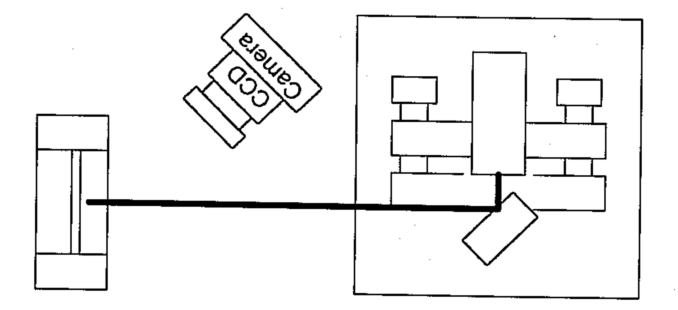
\includegraphics[width=.6\textwidth, angle=1, origin=c]{images/ExternalCavityAlignment.pdf}
	\caption{Justage des externen Resonators \cite{anleitung}.}
	\label{fig:ExternalCavityAlignment}
\end{figure}

Der Injektionsstrom wird so eingestellt, dass die Verstärkung durch induzierte
Emission gerade etwas höher ist als optische Verluste.
Auf der IR Karte zeigt sich das Lasen durch eine Auffächerung des hellen Punktes in ein
Interferenzmuster, welches durch Überlagerung des von der Karte reflektierten
Lichts entsteht.
Diese Auffächerung ist in Abbildung \ref{fig:laser-pattern} dargestellt.

\begin{figure}
	\centering
	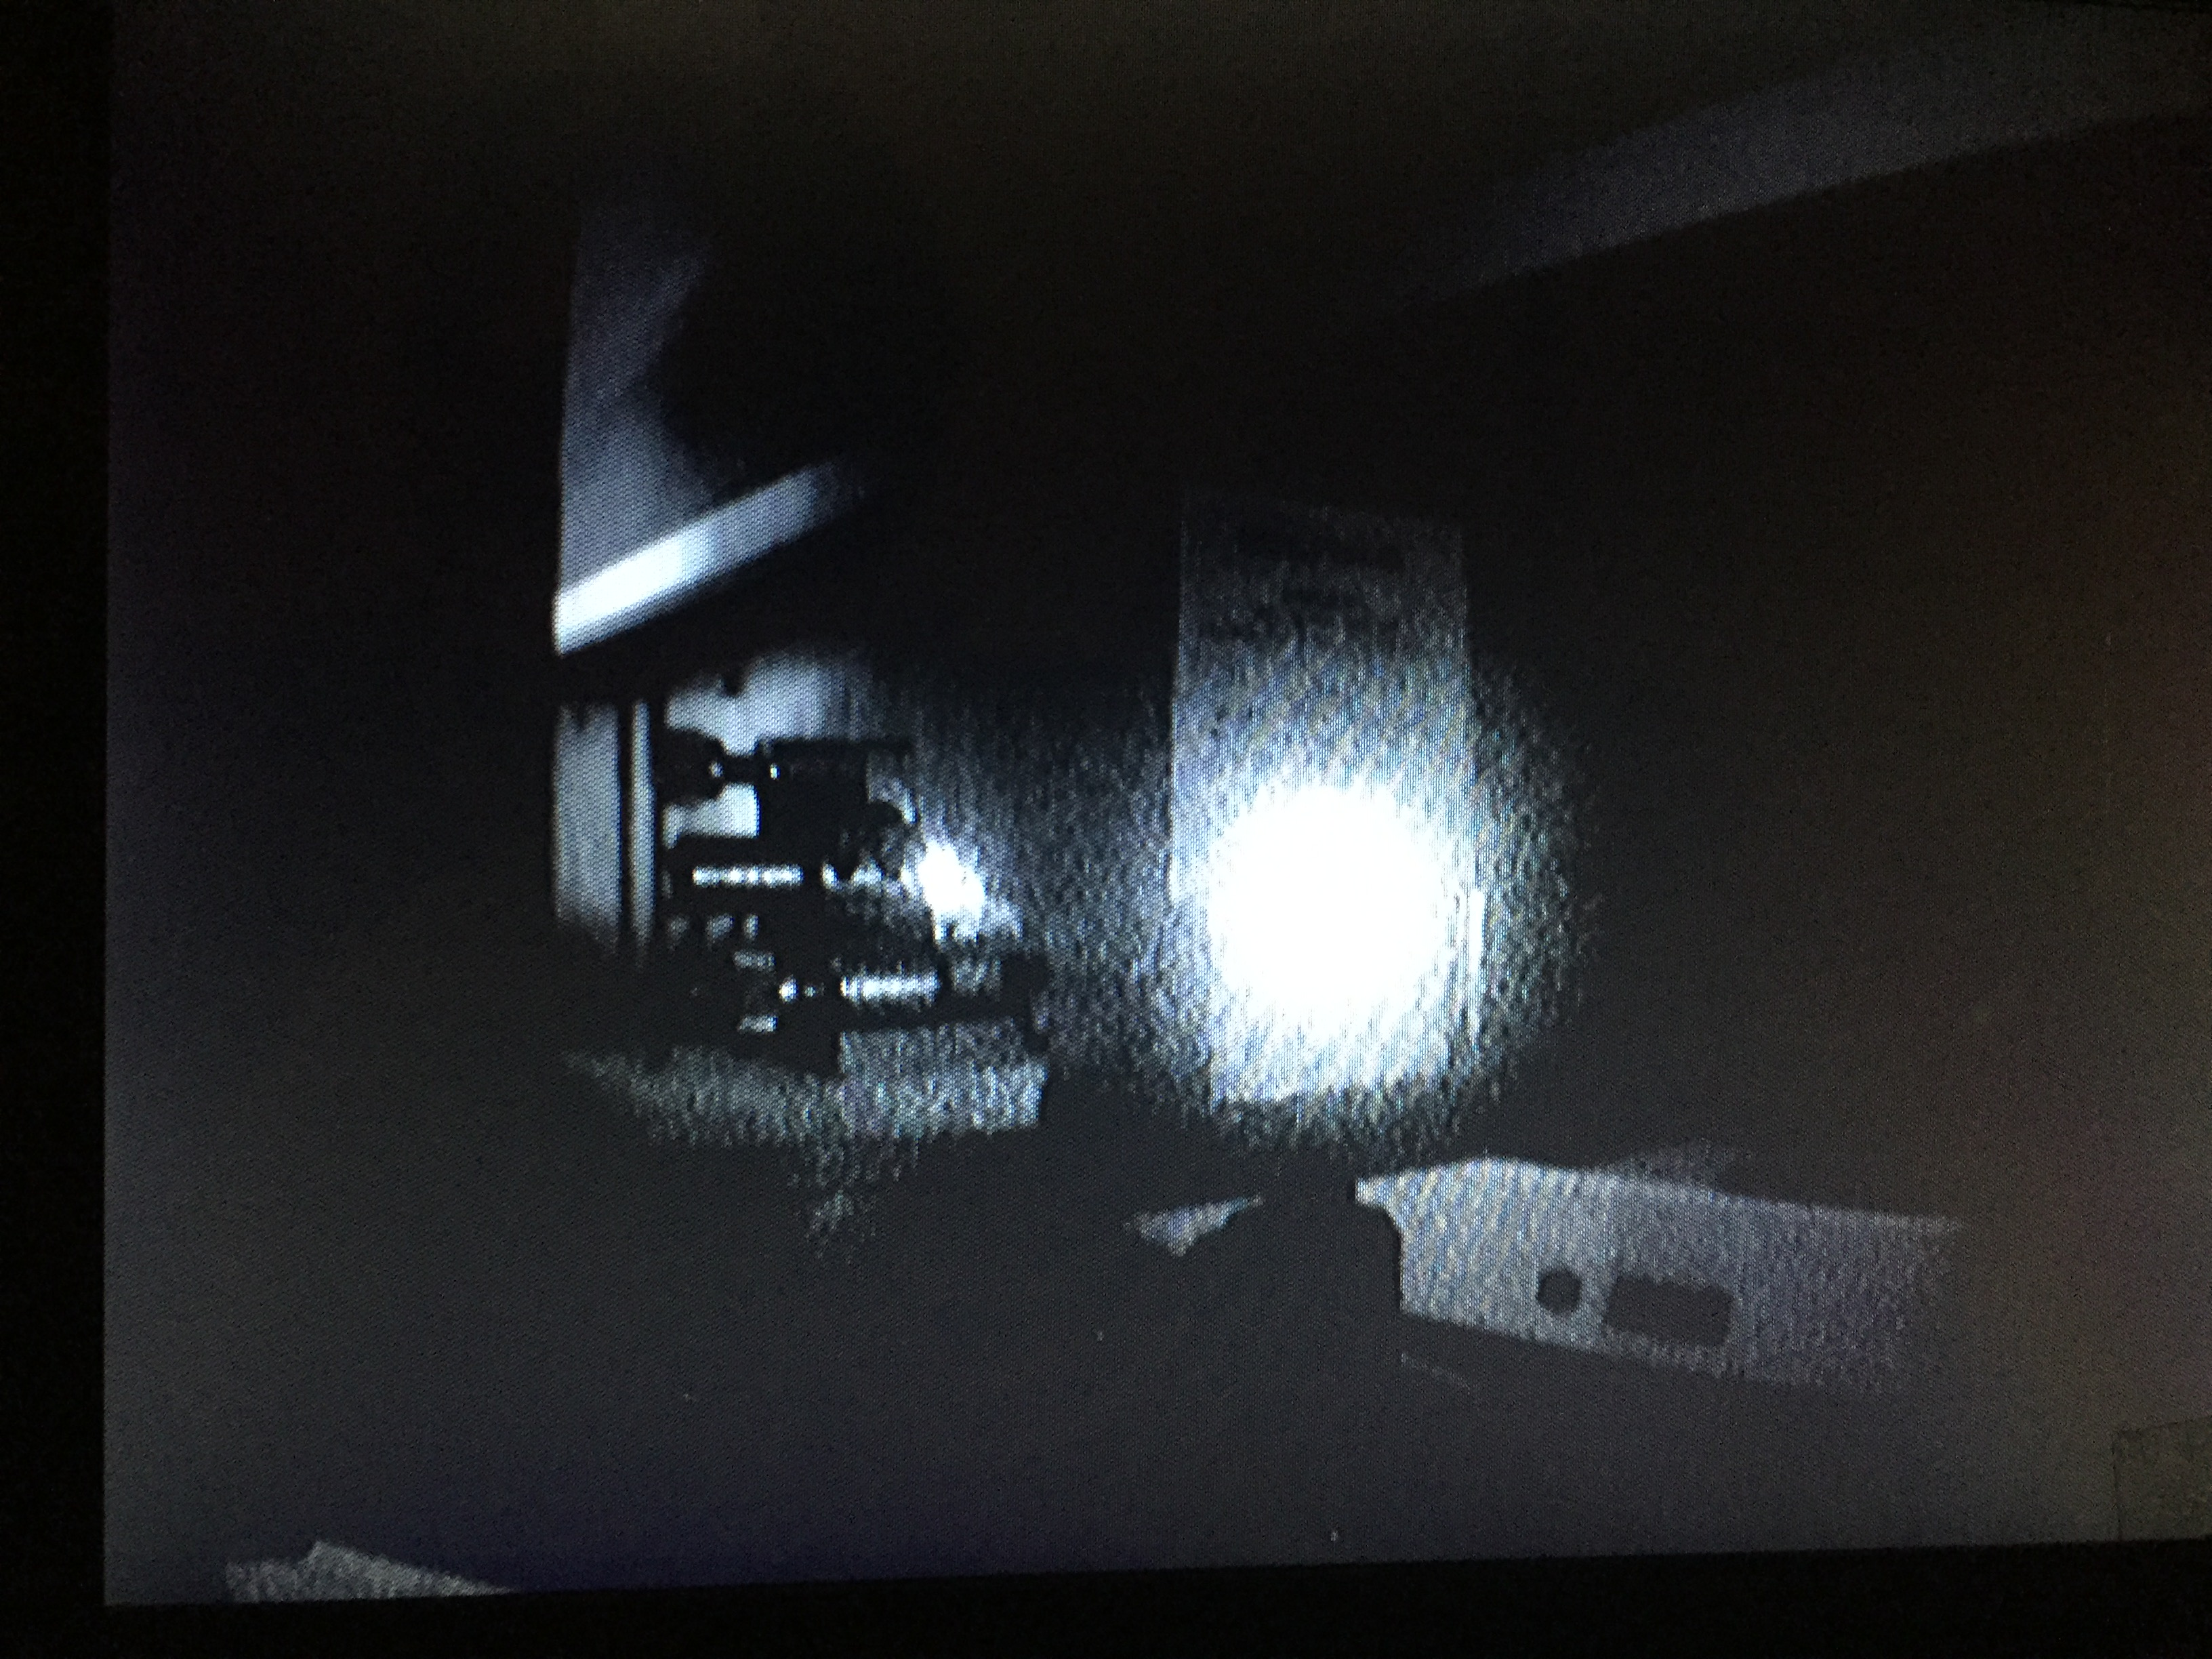
\includegraphics[width=.5\textwidth]{images/laser-pattern.JPG}
	\caption{Auffächerung des Laserpunktes auf der IR Karte.}
	\label{fig:laser-pattern}
\end{figure}

Mit Hilfe des TOP-Drehknopfes der Laserdiode lässt sich der Winkel des Gitters und
dessen Abstand zum Dioden-Chip einstellen.
Wird dieser verändert, lassen sich mehrere Intensitätsmaxima beobachten.
Der Drehknopf wird auf eines dieser Maxima ungefähr in der Mitte der Serie eingestellt.
Im Anschluss lässt sich die Intensität des Injektionsstroms ein wenig herunter regeln,
bis der Laser knapp unter dem Schwellwert zum Lasen ist.
Mit erneuter Justage des TOP-Drehknopfes lässt sich das Lasen der Diode wiederherstellen.
Diese Prozedur wird solange wiederholt, bis eine untere Grenze erreicht ist und der
Strom nicht weiter herunter geregelt werden kann, ohne dauerhaft unterhalb des
Schwellwerts zu bleiben.
Es wurde eine Schwellspannung von \SI{3.36}{\volt} erreicht, die bei einem Widerstand
des Stromgebers von \SI{100}{\ohm} einem Schwellstrom von \SI{33.6}{\milli\ampere} entspricht.


\subsection{Aufnahme des Fluoreszenzspektrums von Rubidium}
\label{sec:Rb-Fluoreszenz}

Für die Beobachtung des Fluoreszenzspektrums von Rubidium ist der Versuchsaufbau
wie in Abbildung \ref{fig:RbFlorescenceSetup} dargestellt anzupassen.
Der Lasterstrahl läuft durch die Rubidiumprobe und trifft auf die IR Karte,
um mögliche Reflexionen im Raum zu vermeiden.
Seitlich an der Apperatur befindet sich eine Bohrung, durch welche das
Fluoreszenzlicht tritt und von der CCD Kamera erfasst wird.

\begin{figure}
	\centering
	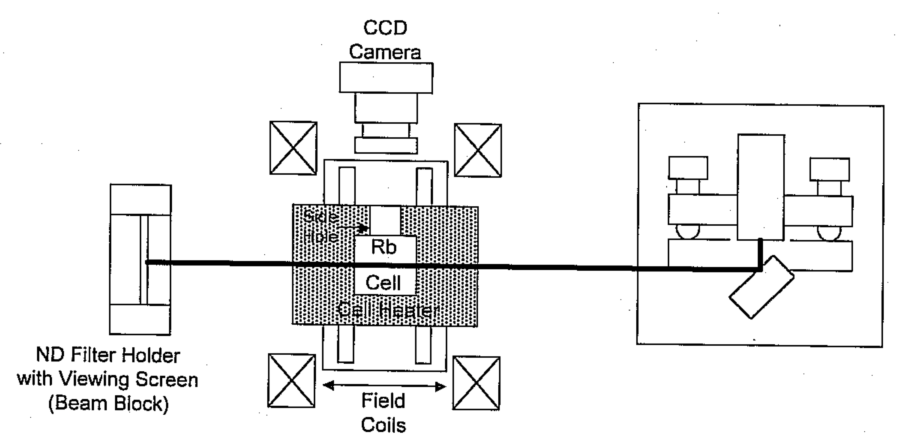
\includegraphics[width=.8\textwidth, angle=1, origin=c]{images/RbFlorescenceSetup.pdf}
	\caption{Schematischer Aufbau zur Beobachtung der Rubidium Fluoreszenz \cite{anleitung}.}
	\label{fig:RbFlorescenceSetup}
\end{figure}

Um Fluoreszenzlicht beobachten zu können, wird der Injektionsstrom etwas über den
bisher eingestellten Grenzstrom eingestellt.
Weiterhin wird die Temperatur de \ce{Rb}-Gases dauerhaft auf \SI{50}{\celsius} geregelt.
Nun wird das Gitter des externen Resonators horizontal mit dem SIDE Drehknopf
verschoben, bis auf dem Bildschirm der CCD Kamera ein heller Streifen sichtbar ist.
Dieser helle Streifen entsteht durch Reemission von Photonen in alle
Raumrichtungen, die zuvor als Laserlicht vom \ce{Rb}-Gas absorbiert wurden.
Dieser helle Streifen ist in Abbildung \ref{fig:RbFlorescence} dargestellt.

\begin{figure}
	\centering
	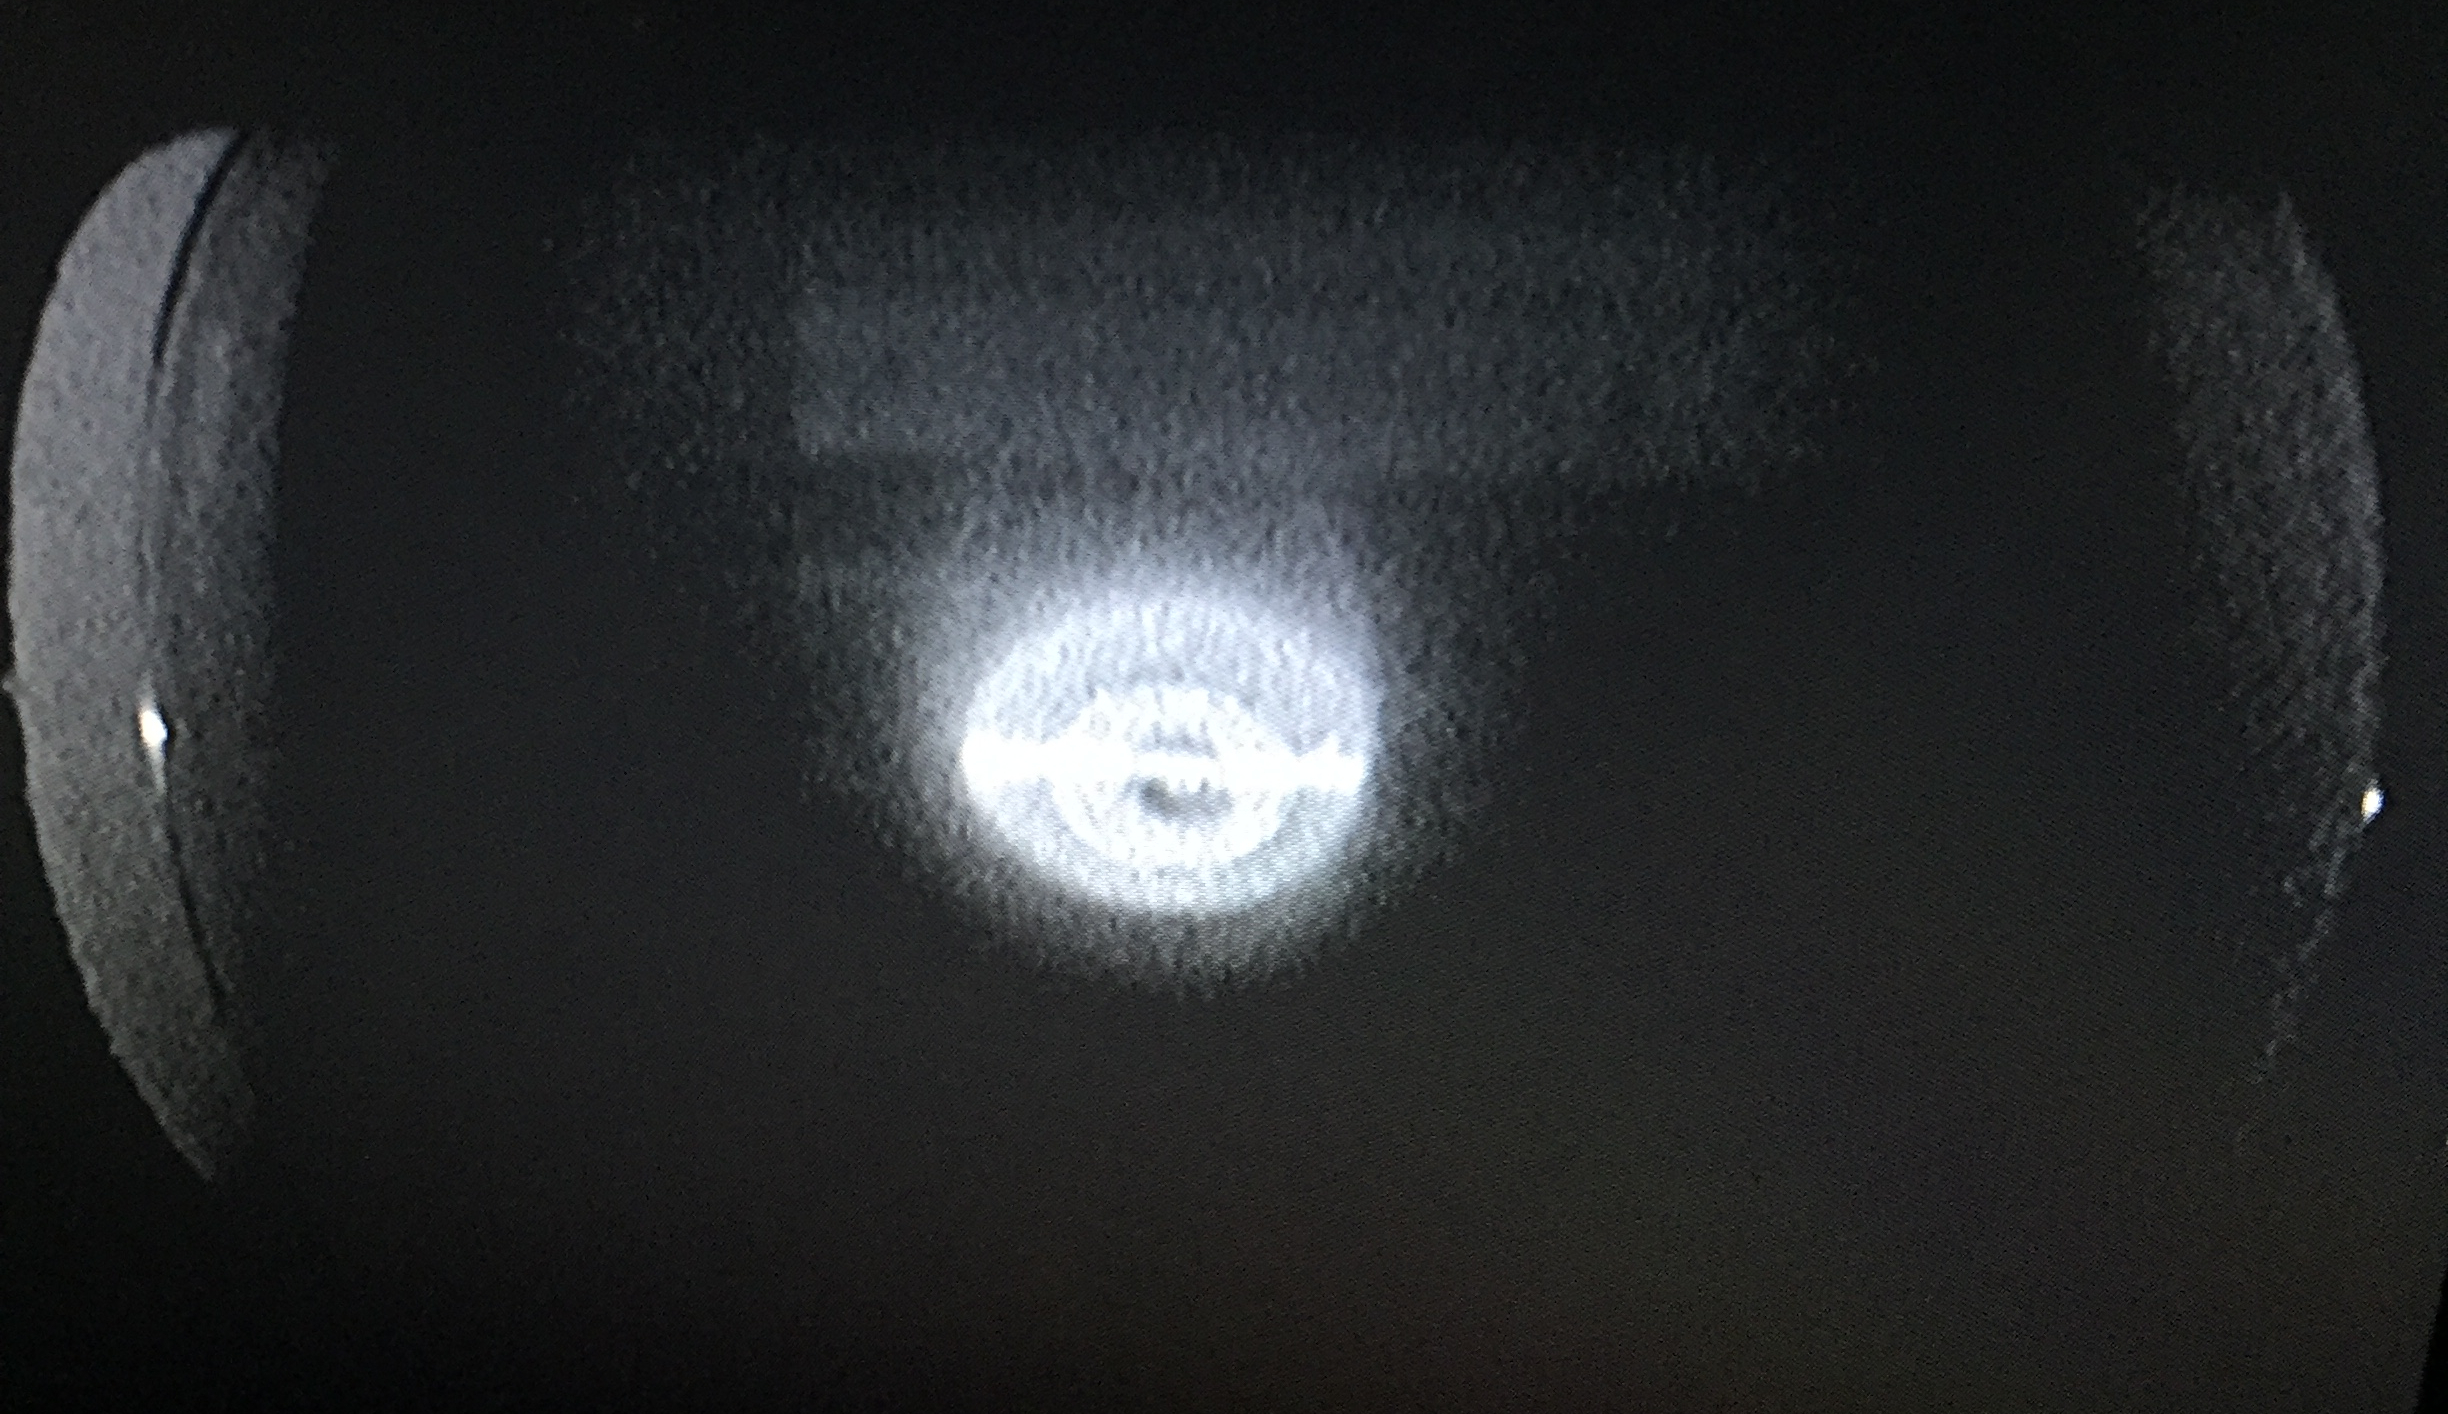
\includegraphics[width=.6\textwidth]{images/florescence.JPG}
	\caption{Mit der CCD-Kamera aufgenommenes Bild der Rubidium Fluoreszenz.}
	\label{fig:RbFlorescence}
\end{figure}

Im Anschluss wird ein RAMP Generator mit einer Frequenz von \SI{10}{\hertz} verwendet,
um das Gitter zu verschieben. Dazu wird der Generator an einen Piezo Kristall
angeschlossen, welcher die Position des Gitters steuert. Weiterhin wird
das Signal des Generators auf einem Oszilloskop angezeigt.
Zusätzlich wird die IR Karte hinter der Rubidiumprobe durch eine Photodiode (PD)
ersetzt, welche ebenfalls an das Oszilloskop angeschlossen wird.
Um zu verhindern, dass die PD durch das Laserlicht gesättigt wird, wird
in den Strahlengang zwischen Laserdiode und Probe ein Neutraldichtefilter plaziert.
Nun wird die Empfindlichkeit der Photodiode auf die maximale Empfindlichkeit
eingestellt, ohne zu saturieren.

\begin{figure}
	\centering
	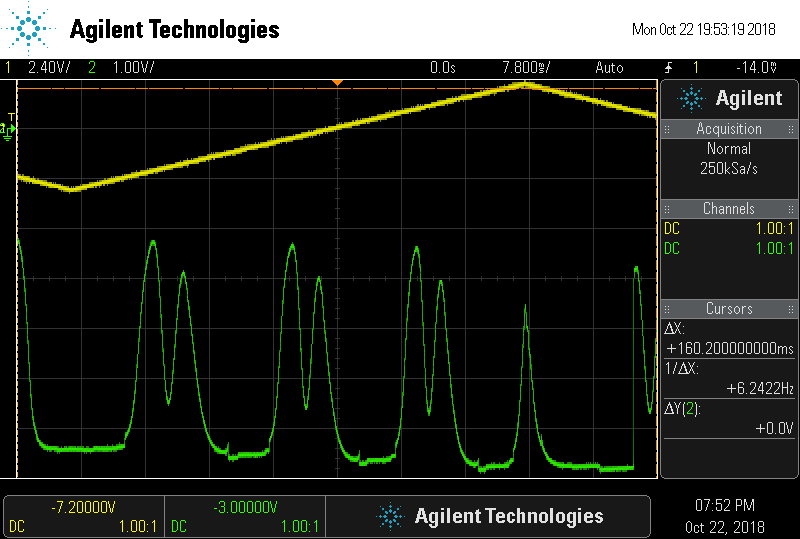
\includegraphics[width=.8\textwidth]{images/first-signal.png}
	\caption{Bildschirmaufnahme des Oszilloskops, welches das Sägezahnsignal des
	RAMP Generators und zwei Absorptionssenkungen aufgrund des Rubidiumdampfes zeigt.}
	\label{fig:first-signal}
\end{figure}

In Abbildung \ref{fig:first-signal} ist das erhaltene Bild des Oszilloskops dargestellt.
Getriggert wurde auf die aufsteigende Flanke des RAMP Generators, welcher als gelbe
Kurve dargestellt ist. In grün ist das Signal der Photodiode dargestellt, welches
im Laufe der Zeit verschiedene Peaks zeigt. Diese Peaks sind (unter Berücksichtigung
der Ausrichtung der y-Achse nach unten) die Absorptionssenkungen des
Laserlichts aufgrund von Anregung von Zuständen des Rubidiumdampfes.
Kleine Zacken im Signal zeigen an, dass es im Laufe eines Durchlaufs des Generators
zu verschiedenen Modensprüngen kommt, sodass dieselben Absorptionssenkungen mehrfach
dargestellt sind.
Durch Variation des Gitter mit Hilfe des SIDE Drehknopfes lassen sich verschiedene
Moden durchfahren. Leider war es bei der Durchführung des Versuchs anfangs nicht möglich,
andere Moden als die zwei in Abbildung \ref{fig:first-signal} dargestellten zu
beobachten.

\subsection{Aufnahme der ersten vier Absorptionslinien von Rubidium}
\label{sec:AbsorptionImproved}

Um mehr als zwei Absorptionssenkungen ohne Modensprünge beobachten zu können, werden im Folgenden
sowohl das Gitter mit Hilfe eines Piezo Kristalls, als auch der Injektionsstrom
mit Hilfe des RAMP Generators variiert.
Der Aufbau wird soweit verändert, dass das Signal des RAMP Generators nun ebenfalls
in den CURRENT MODULATION INPUT gespeist wird.
Es ergibt sich das in Abbildung \ref{fig:second-signal} dargestellte Bild des
Oszilloskops.

\begin{figure}
	\centering
	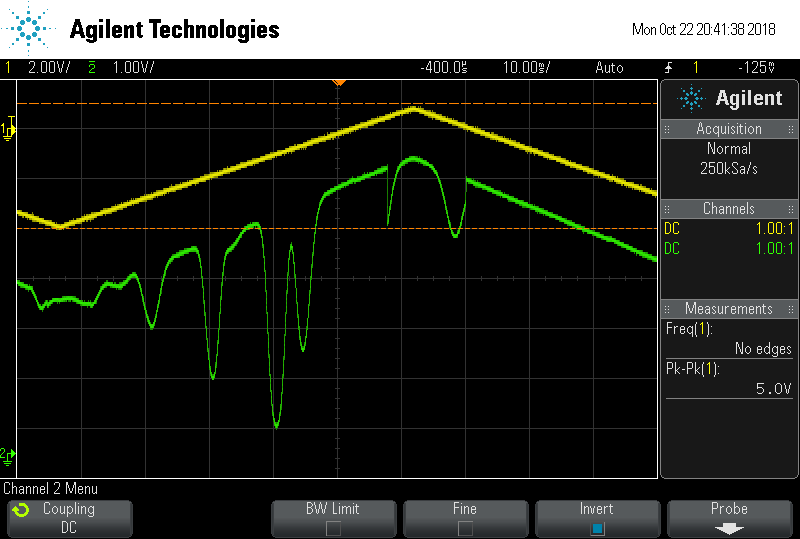
\includegraphics[width=.8\textwidth]{images/second-signal.png}
	\caption{Bildschirmaufnahme des Oszilloskops, welches das Sägezahnsignal des
	RAMP Generators und vier Absorptionssenkungen aufgrund des Rubidiumdampfes zeigt.}
	\label{fig:second-signal}
\end{figure}

Aufgrund der variierten Laserintensität (über den Injektionsstrom) verändert sich
die Hintergrundintensität des Absorptionssignals, sodass die grüne Linie nach
rechts oben zu laufen scheint. Dieser Effekt kann behoben werden, indem eine
Strahlteiler zwischen den ND Filter und die Rubidiumprobe plaziert wird und
ein zweiter Strahlteil auf eine zweite Photodiode trifft. Dieser Aufbau
ist in Abbildung \ref{fig:SetupImproved} dargestellt.

\begin{figure}
	\centering
	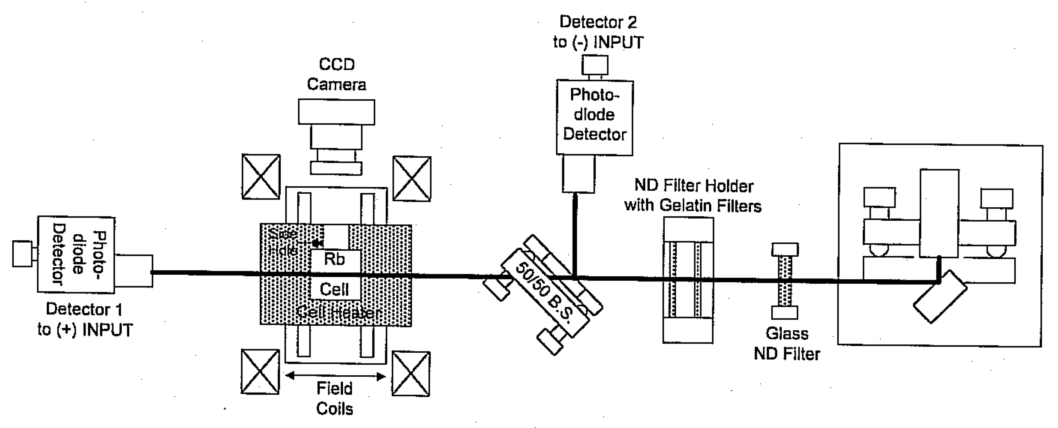
\includegraphics[width=\textwidth, angle=1, origin=c]{images/SetupImproved.pdf}
	\caption{Schematische Skizze des angepassten Versuchaufbaus,
	um Hintergrundintensität mit ein zu beziehen \cite{anleitung}.}
	\label{fig:SetupImproved}
\end{figure}

Beide Photodioden können gegeneinander balanciert werden.
Während der Input der PD hinter der
Rubidiumprobe auf maximaler Balance eingestellt wird, wird die
Balance der zweiten PD langsam erhöht, bis der Effekt der Hintergrundintensität
aufgehoben ist.
Es ergibt sich abschließend das in Abbildung \ref{fig:final-signal} dargestellte
Bild des Oszilloskops.

\begin{figure}
	\centering
	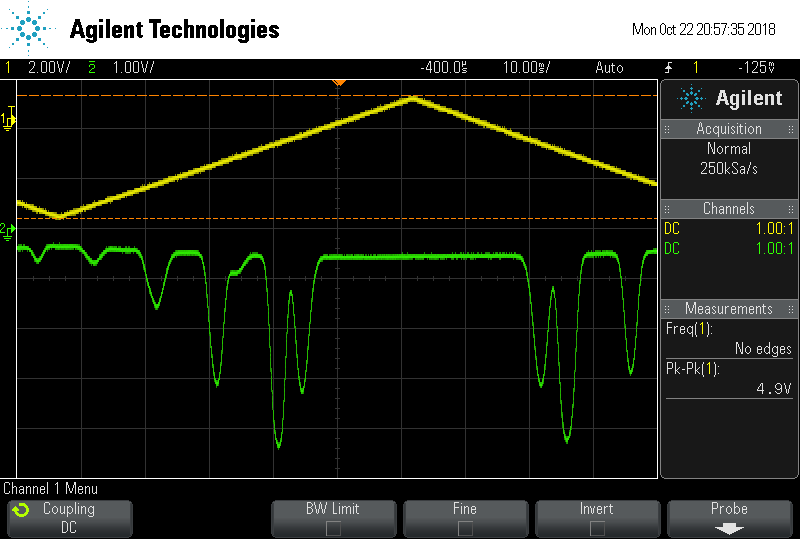
\includegraphics[width=.8\textwidth]{images/final-signal.png}
	\caption{Bildschirmaufnahme des Oszilloskops, welches das Sägezahnsignal des
	RAMP Generators und vier Absorptionssenkungen aufgrund des Rubidiumdampfes zeigt.
	Die variierende Untergrund wurde dabei abgezogen.}
	\label{fig:final-signal}
\end{figure}

\newpage
\section{Auswertung}
\label{sec:Auswertung}

%-------------------------------------------------------------------------------
\subsection{Energiekallibrierung}
\label{sec:Energiekallibrierung}

Für eine Energiekalibrierung wurde das Spektrum der \ce{^{152}Eu}-Quelle
aufgezeichnet. Dies ist in Abbildung \ref{plt:Eu-Spektrum} zu sehen. Die zu
erkennenen Peaks wurden dem erwartetem Europium-Spektrum zugeordnet.
\begin{figure}[htb]
  \begin{subfigure}{0.49\textwidth}
    \centering
    \includegraphics[width=\textwidth]{build/orginal_Eu.pdf}
  \end{subfigure}
  \begin{subfigure}{0.49\textwidth}
    \centering
    \includegraphics[width=\textwidth]{build/orginal_Eu_log.pdf}
  \end{subfigure}
  \caption{Vom Germanium Detektor aufgenommenes Spektrum der Europium Quelle mit
  dekadischer und logarithmischer y-Achse.}
  \label{plt:Eu-Spektrum}
\end{figure}
Anhand der Energien und Bin-Indizes wurde eine lineare Ausgleichsrechnung, in
Abbildung \ref{plt:eichung} zu erkennen, mit Hilfe der Formel
\begin{align*}
  E = m \cdot x + b
\end{align*}
durchgeführt.
\begin{figure}[htb]
  \centering
  \includegraphics[width=0.8\textwidth]{build/kalibation.pdf}
  \caption{Zugeordnete Energien aufgetragen gegen die Bin-Indizes zur
  Kalibrierung des Detektors für die beobachteten Peaks (blau). Zudem ist eine
  lineare Regression der Werte (rot) aufgetragen.}
  \label{plt:eichung}
\end{figure}
Dabei entspricht $x$ der Bin-Indizes. Für die Parameter $m$ und
$b$ ergeben sich:
\begin{align*}
	m &= \SI{0.4204(69)}{\kilo\electronvolt} \\
  b &= \SI{-41.25(1428)}{\kilo\electronvolt}
\end{align*}

\begin{table}
	\centering
	\caption{Gegebene Werte zur Kalibrierung des Germanium-Detektors \cite{anleitung}.}
	\label{tab:anleitung_eu}
	\begin{tabular}{
		S[table-format=1.0]
		S[table-format=2.1]
		S[table-format=1.0]
		}
	\toprule
		{Energie $E\;/\;\si{\si{\kilo\electronvolt}$}} &
		{Bin-Index $i$} &
		{Emis.-Wahr. W} \\
	\midrule
		 122 &  28.6 &  378 \\
		 245 &  7.6 &  691 \\
		 296 &  0.4 &  742 \\
		 344 &  26.5 &  861 \\
		 411 &  2.2 &  1108 \\
		 444 &  3.1 &  1220 \\
		 678 &  2.0 &  1716 \\
		 689 &  0.9 &  1790 \\
		 779 &  12.9 &  1939 \\
		 867 &  4.2 &  2185 \\
		 964 &  14.6 &  2400 \\
		 1005 &  0.6 &  2502 \\
		 1086 &  10.2 &  2703 \\
		 1112 &  13.6 &  2765 \\
		 1299 &  1.6 &  3014 \\
		 1408 &  21.0 &  3501 \\
	\bottomrule
	\end{tabular}
\end{table}
\FloatBarrier

%-------------------------------------------------------------------------------
\subsection{Effizienzmessung des Detektors}
\label{sec:Effizienzmessung}

Zur Berechnung der Detektoreffizienz wurde Formel xy verwendet.  % TODO: Formel einfügen
Dafür wurde zuerst der Raumwinkel anhand Formel xy berechnet. Dabei  % TODO: Formel einfügen
ergibt mit $a = \SI{22.3(10)}{\milli\meter}$ und $r = \SI{22.5(1)}{\milli\meter}$
sich:
\begin{align*}
  \frac{\Omega}{4\pi} = \num{0.01558(34)}
\end{align*}
Dabei wurde $r$ so gewählt, dass der wahrscheinlichste Wechselwirkungspunkt
\SI{1.5}{\centi\meter} innerhalb des Germaniums liegt und der Abstandshalter
zwischen Probe und Detektor \SI{7.31}{\centi\meter} lang ist.
Die Aktivität wurde aus dem Wissen errechnet, dass am 01.10.2000 die Aktivität
der Europium-Probe bei $A = \SI{4130(60)}{\becquerel}$ beträgt. Mithilfe der
Halbwertszeit $t_{\sfrac{1}{2}} = \SI{4943(5)}{\day}$ folgt für den Messtag:
\begin{align*}
    A_\text{Messtag} = A_0 \exp{-\frac{\ln{2} \Delta t}{t_\frac{1}{2}}}=\SI{1633(24)}{\becquerel}
\end{align*}
Der Peakinhalt wurde mit einem Fit durch eine Gaußfunktion der Form
\begin{align*}
	f\left(x\right) = h\cdot \exp{\frac{(x-\mu)^2}{2\sigma^2}} + a
\end{align*}
für jede Energie durchgeführt. Hierbei beschreibt $h$ die Höhe des Peaks, $\mu$
den Mittelwert (um Bin-Indizes der Peaks zu korrigieren), $\sigma$ die
Standardabweichnug und $a$ einen Parameter zur Untergrundberücksichtigung
bezeichnet. Die Parameter der Fits für jedes Bin sind in Tabelle
\ref{tab:gauss_parameter} nachzulesen.

\begin{table}
	\centering
	\caption{Parameter des durchgeführten Gauss-Fits pro Bin. Dabei ist $\mu$ der Mittelwert, $\sigma$ die Standardabweichnug, $h$ die Höhe und a der Energieoffset.}
	\label{tab:gauss_parameter}
	\begin{tabular}{
		S[table-format=1.2] @{${}\pm{}$} S[table-format=1.2]
		S[table-format=1.2] @{${}\pm{}$} S[table-format=1.2]
		S[table-format=1.2] @{${}\pm{}$} S[table-format=1.2]
		S[table-format=1.2] @{${}\pm{}$} S[table-format=1.2]
		}
	\toprule
		\multicolumn{2}{c}{$a$} &
		\multicolumn{2}{c}{$h_i$} &
		\multicolumn{2}{c}{$\mu_i$} &
		\multicolumn{2}{c}{$\sigma_i$} \\
	\midrule
		 68.14 &  1.81 &  18.53 &  2.59 &  384.09 &  1.61 &  11.59 &  2.24 \\
		 28.53 &  0.62 &  36.42 &  209088.64 &  691.33 &  608.71 &  0.26 &  477.23 \\
		 25.80 &  0.56 &  30.13 &  3.79 &  741.15 &  0.20 &  1.39 &  0.20 \\
		 21.02 &  1.00 &  1367.21 &  6.25 &  860.92 &  0.01 &  1.58 &  0.01 \\
		 16.76 &  0.57 &  118.32 &  3.36 &  1108.16 &  0.06 &  1.75 &  0.06 \\
		 16.54 &  0.50 &  7.93 &  3.03 &  1219.87 &  0.74 &  1.69 &  0.76 \\
		 15.21 &  0.42 &  25.36 &  3.66 &  1715.98 &  0.14 &  0.81 &  0.13 \\
		 14.05 &  0.41 &  13.86 &  3.53 &  1789.76 &  0.26 &  0.89 &  0.26 \\
		 12.66 &  0.53 &  180.12 &  2.63 &  1939.14 &  0.04 &  2.39 &  0.04 \\
		 27.24 &  6.78 & -19.01 &  6.23 &  2205.59 &  5.66 &  26.95 &  12.42 \\
		 6.42 &  0.66 &  148.74 &  2.84 &  2398.69 &  0.07 &  3.00 &  0.07 \\
		 5.18 &  0.29 &  7.98 &  1.39 &  2500.53 &  0.50 &  2.48 &  0.51 \\
		 6.44 &  0.62 &  70.59 &  2.39 &  2701.61 &  0.14 &  3.64 &  0.15 \\
		 5.67 &  0.55 &  104.52 &  2.30 &  2766.12 &  0.08 &  3.22 &  0.08 \\
		 3.66 &  0.29 &  9.67 &  1.40 &  3015.25 &  0.42 &  2.57 &  0.44 \\
		 0.69 &  0.45 &  107.38 &  1.70 &  3500.68 &  0.07 &  3.81 &  0.07 \\
	\bottomrule
	\end{tabular}
\end{table}
\FloatBarrier

Aus diesen ergibt sich der Peakinhalt $Z_i$ des Peaks $i$ durch Abintegration
über eine Gaußkurve:
\begin{align*}
  Z_i = \sqrt{2\pi} h_i \sigma_i
\end{align*}

Nun kann aus den gerade berechneten Werten, in Tabelle \ref{tab:det_eff}
aufgelistet, dazu verwenden einen Fit der Form
\begin{align*}
  Q(E) = a \cdot (E - b)^e + c
\end{align*}
durchzuführen. Dabei wurden nur solche Energien betrachtet, die über
\SI{150}{\kilo\electronvolt} liegen. Daraus ergeben sich die Abbildung
\ref{plt:eff} die folgenden Parameter:
\begin{align*}
  a &= -\SI{0.1(23)}{\kilo\electronvolt\per\becquerel} \\
  b &= \SI{2(12)}{\kilo\electronvolt} \\
  c &= \SI{6(20)}{\raiseto{-1}\becquerel} \\
  e &= \num{0.5(20)}
\end{align*}

\begin{figure}[htb]
  \centering
  \includegraphics[width=0.8\textwidth]{build/efficiency.pdf}
  \caption{Fit zur Effizienzbestimmung des Detektors anhand der zuvor
  berechneten Werten der Efizienz anhand der Energien.}
  \label{plt:eff}
\end{figure}

\begin{table}
	\centering
	\caption{Peakhöhe, Energie und Detektoreffizenz als Ergebnis des Gaußfits.}
	\label{tab:det_eff}
	\begin{tabular}{
		S[table-format=1.2] @{${}\pm{}$} S[table-format=1.2]
		S[table-format=1.2]
		S[table-format=1.2] @{${}\pm{}$} S[table-format=1.2]
		}
	\toprule
		\multicolumn{2}{c}{$Z_i$} &
		{E_i} &
		\multicolumn{2}{c}{$Q \ \si{becquerel}$} \\
	\midrule
		 538.41 &  128.48 &  120.24+/-0.68 &  0.74 &  0.18 \\
		 24.06 &  144843.44 &  249.41+/-255.92 &  0.12 &  749.00 \\
		 104.94 &  20.29 &  270.36+/-0.08 &  10.31 &  2.00 \\
		 5423.10 &  38.12 &  320.71+/-0.00 &  8.04 &  0.13 \\
		 519.47 &  22.69 &  424.66+/-0.02 &  9.28 &  0.43 \\
		 33.65 &  19.80 &  471.63+/-0.31 &  0.43 &  0.25 \\
		 51.61 &  11.13 &  680.21+/-0.06 &  1.01 &  0.22 \\
		 30.91 &  12.06 &  711.23+/-0.11 &  1.35 &  0.53 \\
		 1079.54 &  24.38 &  774.04+/-0.02 &  3.29 &  0.09 \\
		-1284.03 &  725.94 &  886.06+/-2.38 & -12.02 &  6.80 \\
		 1118.21 &  33.15 &  967.25+/-0.03 &  3.01 &  0.10 \\
		 49.64 &  13.42 &  1010.07+/-0.21 &  3.25 &  0.88 \\
		 644.04 &  33.97 &  1094.61+/-0.06 &  2.48 &  0.14 \\
		 844.48 &  28.90 &  1121.73+/-0.03 &  2.44 &  0.09 \\
		 62.29 &  13.92 &  1226.48+/-0.18 &  1.53 &  0.34 \\
		 1024.99 &  25.27 &  1430.57+/-0.03 &  1.92 &  0.05 \\
	\bottomrule
	\end{tabular}
\end{table}
\FloatBarrier

%-------------------------------------------------------------------------------
\subsection{Bestimmung der Detektoreigenschaften}
\label{sec:Detektoreigenschaften}
Für diesen Teil der Auswertung wurde das Spektrum eines Cäsium-Strahlers, in
Abbildung \ref{plt:Cs} zu sehen, aufgenommen.

\begin{figure}
  \begin{subfigure}{0.49\textwidth}
    \centering
    \includegraphics[width=\textwidth]{build/spektrum_Cs.pdf}
  \end{subfigure}
  \begin{subfigure}{0.49\textwidth}
    \centering
    \includegraphics[width=\textwidth]{build/spektrum_Cs_log.pdf}
  \end{subfigure}
  \caption{Vom Detektor aufgenomenes Spektrum der Cäsium-Quelle, dargestellt
  mit dekadischer und logarithmischer y-Achse.}
  \label{plt:Cs}
\end{figure}
Hier wurden die charakteristischen
Peaks des Spektrums (Rückstreu- und Vollenergiepeak, sowie die Comptonkante)
identifiziert. Die Zuordnung dieser sind in \ref{tab:Cs_char} nachzulesen. Der
Theoriwert des Vollenergiepeaks liegt bei \SI{661.59}{\kilo\electronvolt}
\cite{theorie}.
\begin{table}[htb]
	\centering
  \begin{tabular}{c
    S[table-format=4.0]
    S[table-format=3.2]}
    \toprule
    {} & {Index $i$} & {Energie $E_i$ / keV} \\
    \midrule
    Rückstreupeak & 511 & 173,59 \\
    Compton-Kante & 1174 & 452,63 \\
    Vollenergiepeak & 1648 & 651,63 \\
    \bottomrule
  \end{tabular}
  \caption{Charakteristische Peaks des Cs-Strahlers.}
  \label{tab:Cs_char}
\end{table}

Eine Berechnung der Theoriwerte für Rückstreupeak und Comptonkante durch die
Energie des Vollenergiepeaks $E_{\text{Voll}}$ normiert auf $m_0\:c^2$ ergibt:
\begin{align*}
  E_\text{Compton, Theo} &= \frac{2\epsilon}{1+2\epsilon}\cdot E_\text{Voll} = \SI{1136.32}{\kilo\electronvolt} \\
  E_\text{Rück, Theo} &= \frac{1}{1+2\epsilon}\cdot E_\text{Voll} = \SI{659.88}{\kilo\electronvolt}
\end{align*}
Diese Werte weichen wie folgt von den gemessenen Werten ab:
\begin{align*}
  \Delta E_\text{Compton} &= \SI{60.19}{\percent} \\
  \Delta E_\text{Rück} &= \SI{73.69}{\percent}
\end{align*}

Um zu überprüfen, ob der Vollenergiepeak eine Gaussform annimmt, wird eine
rechte (r) und eine linke (l) Flanke mithilfe einer linearen Regression
angenommen. Daraus ergeben sich die Parameter:
\begin{align*}
  a_\text{l} &= \num{0.0042(7)} \quad a_\text{r} = \num{-0.0039(6)} \\
  b_\text{l} &= \num{1640.6(6)} \quad b_\text{r} = \num{1655.2(6)}
\end{align*}
Durch Hinzunahme der Formel
\begin{align*}
	\Delta_\text{x} = m_\text{r}xh + b_\text{r} - \left(m_\text{l}xh + b_\text{l}\right)\ \text{mit}\ h \in \left\{\num{0.1}; \num{0.5}\right\}
\end{align*}
kann die Halbwerts- und die Zehntelbreite bestimmt werden. Daraus ergab sich:
\begin{align*}
  \Delta_{1/2} &= \SI{-38.3(5)}{\kilo\electronvolt} \\
	\num{1.823} \cdot \Delta_{1/2} &= \SI{-35.9(9)}{\kilo\electronvolt} \\
  \Delta_{1/10} &= \SI{-35.7(4)}{\kilo\electronvolt}
\end{align*}
Wird nun das Verhältnis zwischen den beiden unteren asdf  % TODO
betrachtet, so erhält man hier eine Abweichung zum ermittelten Wert von
$\Delta_{1/10}$ von \SI{5}{\percent}.

Im letzten Schritt dieses Auswertungsteils wird der Inhalt des Compton-Kontinuums
und des Vollenergiepeaks mit der Absorptionswahrscheilichkeit des Compton- und
Photoeffektes verglichen. Dafür wird die Formel
\begin{align*}
	p = 1 - \exp\left(-\mu l\right)
\end{align*}
mit der Länge des Detektors $l = \SI{3.9}{\centi\meter}$ und dem
Absorptionskoeffizienten $\mu$ verwendet. Dabei ergeben sich die
Absorptionskoeffizienten aus Abbildung \ref{plt:Cs_abs} zu:
\begin{align*}
	\mu_\text{Compton} &= \SI{111}{\per\centi\meter} & p_\text{Compton} &= \SI{111}{\percent} \\
	\mu_\text{Photo} &= \SI{111}{\per\centi\meter} & p_\text{Photo} &= \SI{111}{\percent}
\end{align*}

\begin{figure}
  \begin{subfigure}{0.49\textwidth}
    \centering
    \includegraphics[width=\textwidth]{build/Cs.pdf}
  \end{subfigure}
  \begin{subfigure}{0.49\textwidth}
    \centering
    \includegraphics[width=\textwidth]{build/Cs_log.pdf}
  \end{subfigure}
  \caption{Vollenergiepeak und Compton-Kontinuum des Cs-Spektrums.}
  \label{plt:Cs_abs}
\end{figure}

\subsection{Aktivitätsbestimmung anhand eines Spektrums}
\label{sec:Aktivitätsbestimmung}

\subsection{Identifizierung eines aktiven Nuklids per Spektrum}
\label{sec:Nuklidbestimmung}


\section{Diskussion}
\label{sec:Diskussion}
Die Durchführung der Energiekalibrierung ist wie in Abbildung \ref{plt:eichung}
zu sehen ohne nennenswerte UNsicherheiten durchgeführt worden. Dies spricht
dafür, dass die Zuordnung der Peaks zu den entsprechenden Energien korrekt ist.

Bei Berechnung der Aktivität am Messtag und des Raumwinkels wurden bis auf kleine
Unsicherheiten realistische Werte erhalten. Der Fit mithilfe einer gaußförmigen
Funktion ergab durchweg konsistente Parameter. Dabei ist die Unsicherheit auf
den zweiten Wert in Tabelle \ref{tab:gauss_parameter} und die dadurch
berechenten Werten in Tabelle \ref{tab:gauss_parameter} sehr hoch, was auf eine
nicht korrekte Zuornung des entsprechenden Peaks hinweisen könnte. Ebenso ist
diese Begründung in dem jeweils in den Tabellen auftretenden negativen Wert
anzuführen.

Die Bestimmung des Nuklid von Barium oder Antimon zeigt bei Betrachtung der
berechneten Aktivität und die geringen Unsicherheiten der Gauß-Fit Parameter
eine ausreichend gute Zuordnung der Peaks zu den Energien. Bei der Berechnung
der Aktivität konnten zwei Werte nicht berechnet werden, da sie die Bedingung
$E_\gamma > \SI{150}{\kilo\electronvolt}$ nicht erfüllen.


Beim letzten Schritt der Auswertung, dem identifizieren eines aktiven Nuklids
anhand eines Spektrums, ist die Betrachtung der Emissionslinien in diesem Fall
einfach gehalten, da nur zwei Energien mit deutlich erhöhter Zählrate auftreten.
Dabei ist de genaue Unterscheidung zwischen Wismut und Titan nicht möglich, da
deren Emissionslinien sehr nah bei einander liegen.


\nocite{*}
\printbibliography

\end{document}
